%------------------------------------------
%       $Id: GMT_Appendix_E.tex,v 1.7 2005-10-25 13:30:23 remko Exp $
%
%       The GMT Documentation Project
%       Copyright 2000-2005.
%       Paul Wessel and Walter H. F. Smith
%------------------------------------------
%
\chapter{Predefined bit and hachure patterns in \gmt}
\index{Attributes!fill!pattern}
\index{Fill!attributes!pattern}
\index{Pattern}
\thispagestyle{headings}

\GMT\ provides 90 different bit and hachure patterns that can be
selected with the \Opt{Gp} or \O pt{GP} option in most plotting programs.
The left side of each image was created using \Opt{Gp}, the right side
shows the inverted version using \Opt{GP}.
These patterns are reproduced below at 300 dpi.

\begin{center}
%\epsfig{figure=eps/GMT_App_E.eps}
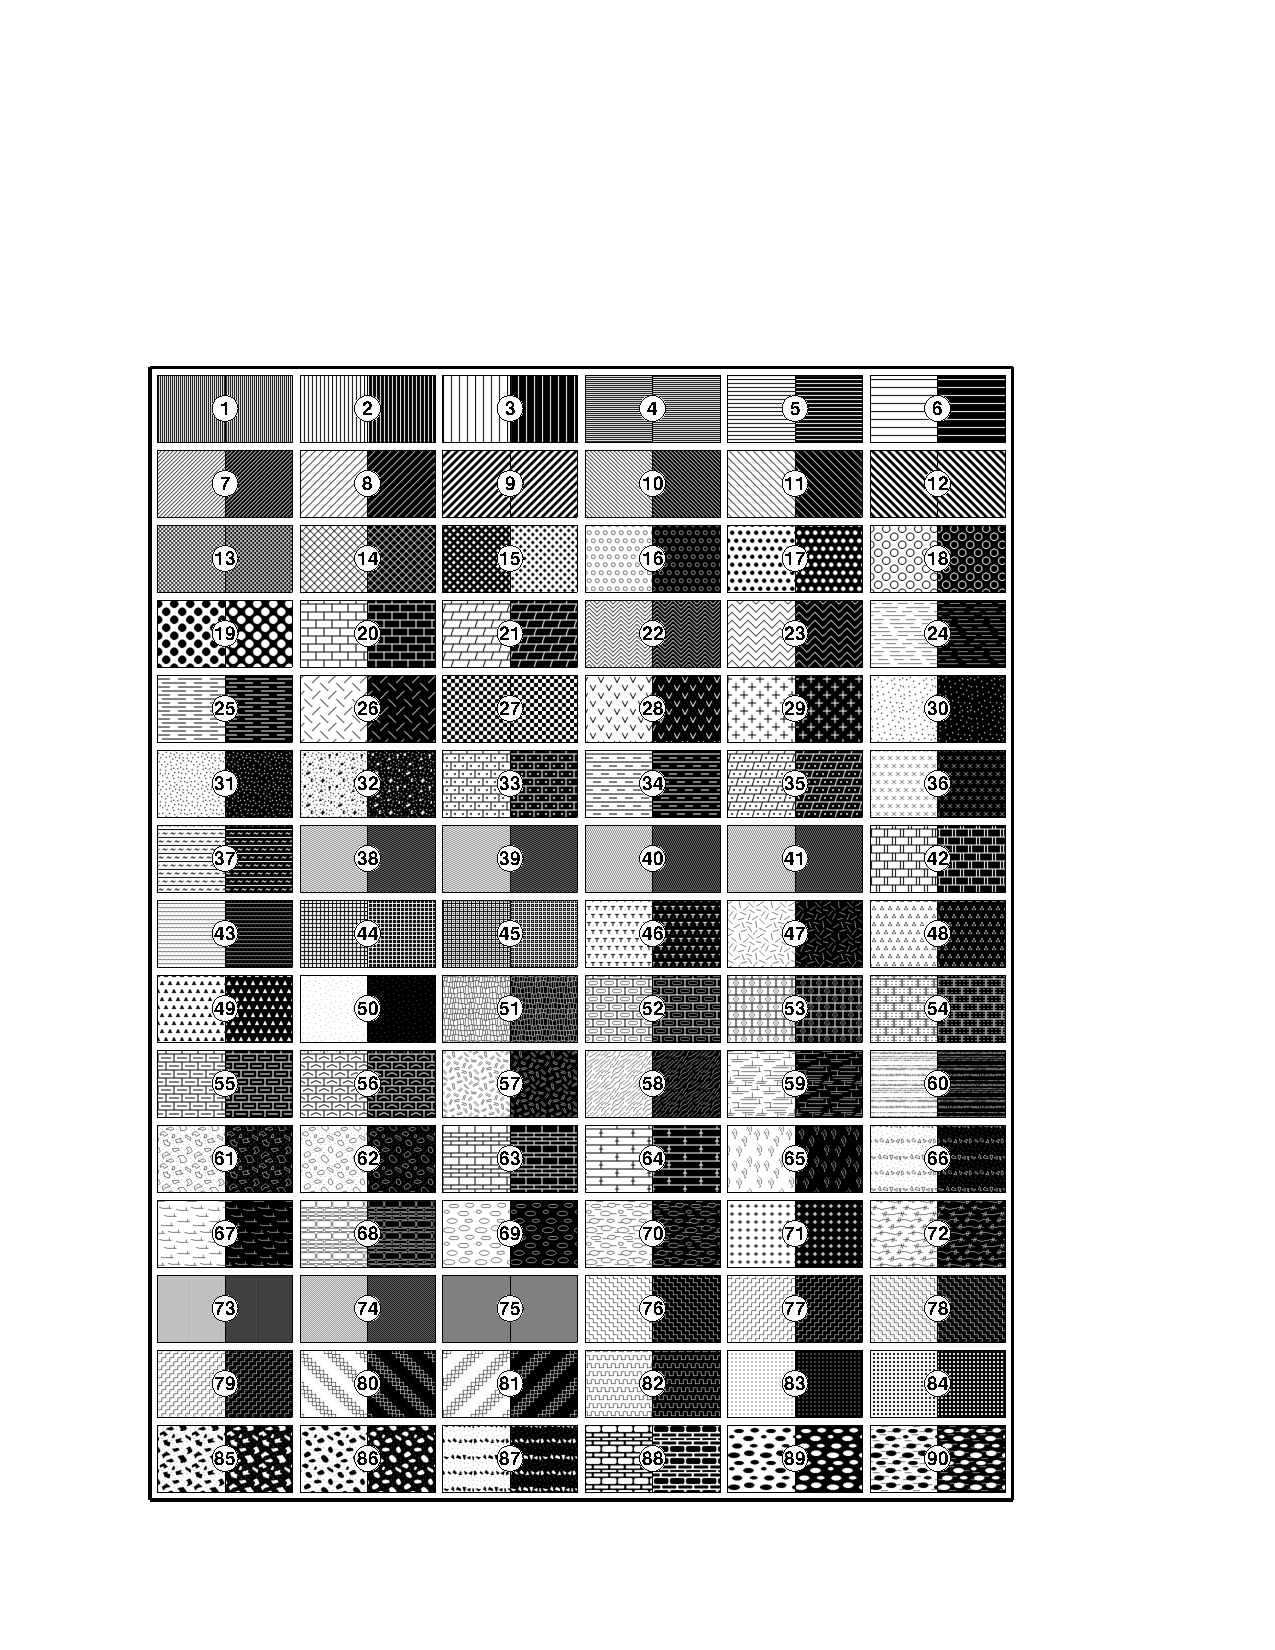
\includegraphics{eps/GMT_App_E}
\end{center}
